\section{IDE-Specific Project Configuration}

This section describes how to create a project for developing with the 
Kieker sources in different IDEs.

\subsection{Netbeans}

You create a Netbeans project for the Kieker trunk as follows:

\begin{compactenum}
\item File->New Project\ldots and select \textit{Java Free-Form Project} and 
follow the wizard and answer the dialogs as follows:

\begin{compactenum}
\item \textbf{Name and Location (Fig.~\ref{fig:nb:location}):} %

Select Kieker's trunk/ directory as the project location and th wizard will %
complete the missing information based on the existing build.xml file.

\begin{figure}[H]\centering
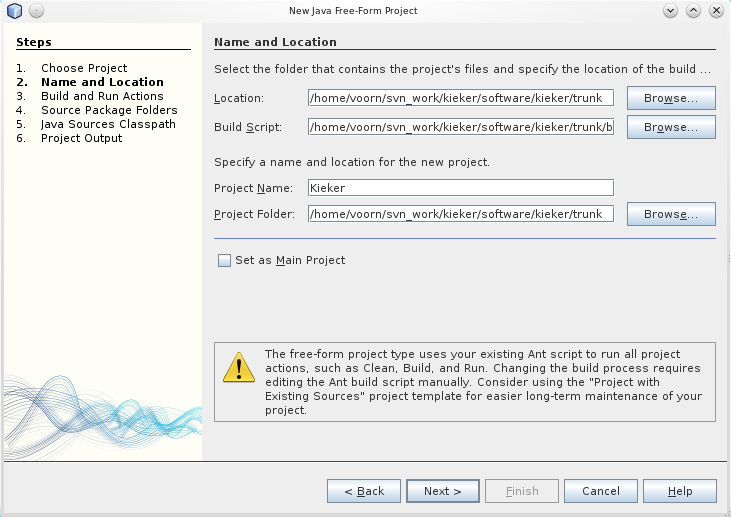
\includegraphics[scale=0.5]{figures/netbeans-NameAndLocation}
\caption{}
\label{fig:nb:location}
\end{figure}

\item \textbf{Build and Run Actions (Fig.~\ref{fig:nb:buildRun}):} %

Complete the information as shown in Fig.~\ref{fig:nb:buildRun}.

\begin{figure}[H]\centering
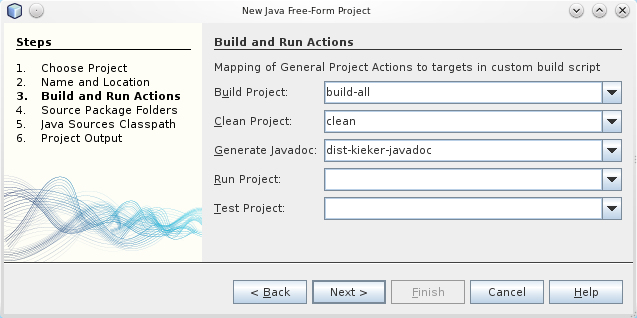
\includegraphics[scale=0.5]{figures/netbeans-BuildAndRun}
\caption{}
\label{fig:nb:buildRun}
\end{figure}

\item \textbf{Source Package Folders (Fig.~\ref{fig:nb:sourcePackageFolders}):} %

\textbf{Add} alls subdirectories of src/ and all subdirectories of test/ (except META-INF/) to 
the list of \textit{Source Package Folders}. \textbf{Remove all \textit{Test Package Folders} entries.}

\begin{figure}[H]\centering
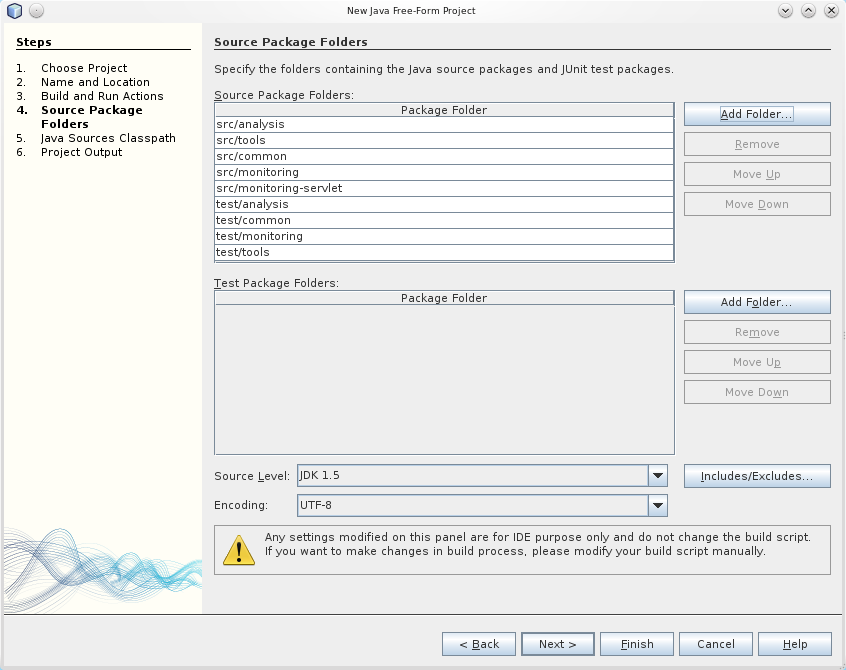
\includegraphics[scale=0.5]{figures/netbeans-SourcePackageFolders}
\caption{}
\label{fig:nb:sourcePackageFolders}
\end{figure}

\item \textbf{Java Sources Classpath (Fig.~\ref{fig:nb:sourcesclasspath}):} %

\textbf{\underline{Un}check} the option \textit{Separate Classpath for Each Source Package Folder} and %
\textbf{add} all .jar files included in he lib/ directory.

\begin{figure}[H]\centering
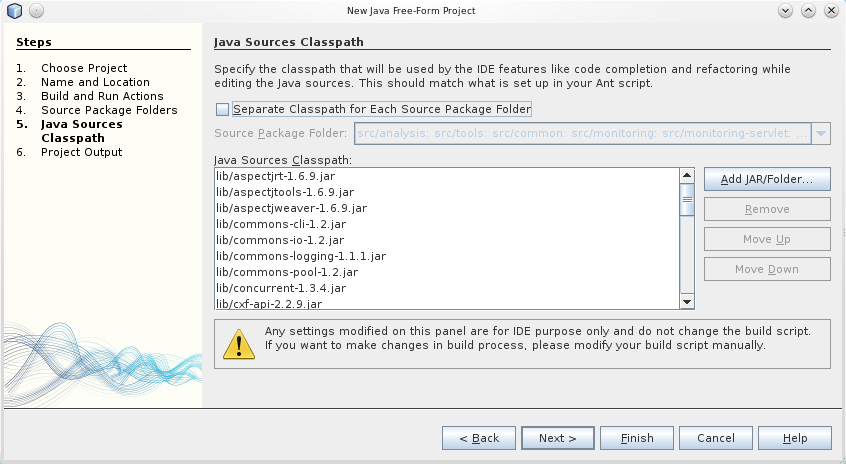
\includegraphics[scale=0.5]{figures/netbeans-SourcesClasspath}
\caption{}
\label{fig:nb:sourcesclasspath}
\end{figure}

\end{compactenum}
\end{compactenum}



\subsection{Eclipse}